%label:"fig:intersectionoftropicalcurves"
%author:JeffHicks
%name:"intersection of tropical curves"
%type:"figure"
%parent:"art_tropicalGeometryIntersection"
%caption:"We compute the intersection between the two tropical curves drawn on the left hand side by first taking a slight perturbation so that they intersect transversely. The set obtain in the limit as the perturbations go to zero is independent of the choice of transverse perturbation. In this setting, the intersection of two tropical lines is a point."
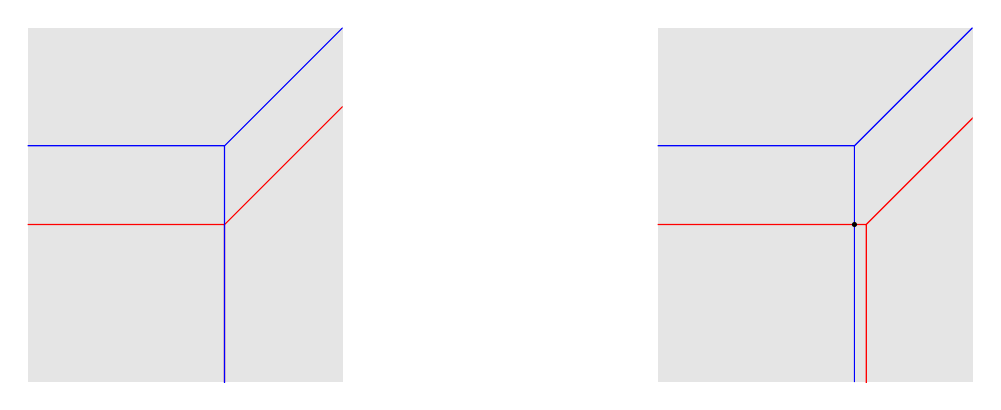
\begin{tikzpicture}\begin{scope}[shift={(0,0)}]

        \fill[gray!20]  (1.5,2) rectangle (-2.5,-2.5);
        \clip  (1.5,2) rectangle (-2.5,-2.5);
                \draw[blue] (-2.65,0.5) -- (0,0.5) -- (0,-2.5) (1.5,2) -- (0,0.5);
                \draw[red] (-3,-0.5) -- (0.15,-0.5) -- (0.15,-3) (1.65,1) -- (0.15,-0.5);
                
        \node[circle, fill=black, scale=.2] at (0,-0.5) {};
        \end{scope}
        
                    \begin{scope}[shift={(-9,1)}]
                    \fill[gray!20]  (2.5,1) rectangle (-1.5,-3.5);
                    \clip  (2.5,1) rectangle (-1.5,-3.5);
        \draw[red] (-2,-1.5) -- (1,-1.5) -- (1,-3.5) (2.5,0) -- (1,-1.5);
                    \draw[blue] (-2.5,-0.5) -- (1,-0.5) -- (1.0001,-4) (2.5,1) -- (1,-0.5);
        
        \end{scope}
                \end{tikzpicture}
        